\bookchapter{Team play under the rules}\label{ch:rc4}

\section*{Explanation}
A team of robots is more than the sum of its robots. Three things make the difference between five robots that happen to be on the same field and a team: \textbf{roles} (who does what), \textbf{communication} (who knows what), and the \textbf{rules} that limit both. This chapter looks at the three together, because in the HSL the rules shape the design: you may send only a limited number of messages, only a limited number of robots may stand in the goal area, and every foul costs a robot.

\section*{Roles and the problem of flapping}
A typical team has a few roles: the \textbf{goalkeeper} (the only robot allowed to use its hands inside its own penalty area), the \textbf{striker} that goes for the ball, \textbf{supporters} that walk to useful positions near the ball, and \textbf{defenders}. The simplest striker rule is: \emph{the robot that is nearest to the ball is the striker.}

This rule has a problem that every team meets. The distance to the ball is measured with noise (Chapter~\ref{ch:ctl6}: far away a pixel is metres). When two robots are about equally far from the ball, the nearest one changes from one cycle to the next, and so does the role: both robots start to walk to the ball, stop, turn... The role \textbf{flaps}. The cure is \textbf{hysteresis} (the idea of a thermostat that does not switch at every small change): the current striker stays striker unless another robot is better by a margin $h$:
\[
\text{change the striker to robot } j \iff d_j < d_{\text{striker}} - h .
\]

\begin{center}
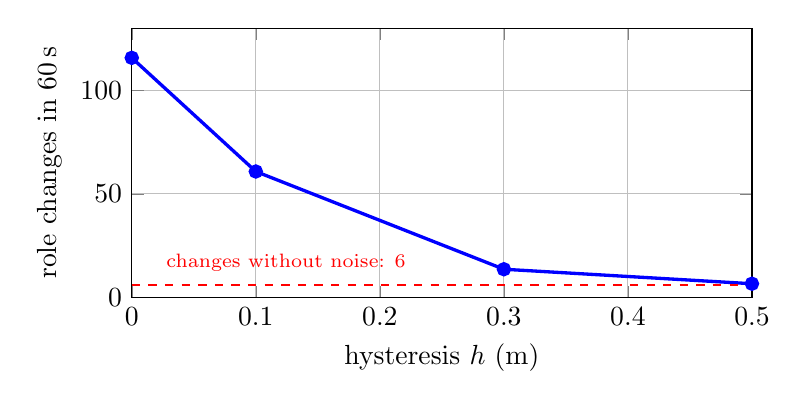
\begin{tikzpicture}
\begin{axis}[width=0.78\linewidth,height=5cm,xlabel={hysteresis $h$ (m)},ylabel={role changes in 60\,s},xmin=0,xmax=0.5,ymin=0,ymax=130,xtick={0,0.1,0.2,0.3,0.4,0.5},grid=both]
 \addplot[blue,very thick,mark=*] coordinates {(0,115.7)(0.1,60.8)(0.3,13.6)(0.5,6.6)};
 \addplot[red,dashed] coordinates {(0,6)(0.5,6)};
 \node[font=\scriptsize,red,anchor=south west] at (axis cs:0.02,8) {changes without noise: 6};
\end{axis}
\end{tikzpicture}
\captionof{figure}{Role changes in a simulation with three robots, a ball that moves along a Lissajous path, and distance noise of $0.15$\,m (standard deviation), $10$ decisions per second for $60$\,s, mean of $200$ runs. Without hysteresis the striker changes about $116$ times, although the ideal (noise-free) decision changes only $6$ times. A margin of $0.3$--$0.5$\,m brings it close to the ideal.}
\end{center}

The decision procedure, in Python, with the margin as the only parameter:
\begin{verbatim}
def choose_striker(current, dists, h=0.3):
    """dists: estimated distance of each robot to the ball (m)."""
    best = min(range(len(dists)), key=lambda i: dists[i])
    if best != current and dists[best] < dists[current] - h:
        return best
    return current
\end{verbatim}
The price of the margin is a \emph{delay}: a robot that is really better by less than $h$ does not get the role. This is a good trade, because a robot that wastes two seconds turning around is worse than a striker that is $0.3$\,m farther away. Note also that the decision must be \textbf{the same on all robots}: either one robot decides for everybody, or all robots use the same inputs (shared ball and positions) and the same rule. Otherwise two robots can both believe that they are the striker.

\section*{The rules that shape the behaviour}
The rules of Chapter~\ref{ch:rc2} are a list of things the behaviour must \emph{avoid}. A few examples from the draft:
\begin{itemize}[nosep]
 \item \textbf{At most three robots of a team} may be in the team's own goal area during \emph{set} and \emph{playing}; an additional robot that enters it is penalised for illegal position (a robot that was pushed in has $5$\,s to leave).
 \item \textbf{Ball holding}: a robot that keeps the ball under control for more than $5$\,s ($10$\,s for the goalkeeper in its penalty area) is penalised. The dribbling behaviour needs a timer.
 \item \textbf{Local game stuck}: if the ball did not move for $10$\,s and robots stand around it, the nearest one is penalised; the same robot must \emph{kick}, not wait.
 \item \textbf{Pushing}: contact that destabilises the opponent, or that lasts longer than $5$\,s. The walking planner must avoid walking \emph{through} an opponent: obstacle avoidance is a rule, not a nicety.
 \item \textbf{Wide stance} (longer than $10$\,s) and \textbf{playing with hands}: hands may be used only by the goalkeeper in its own penalty area.
 \item \textbf{Kick-off}: in \emph{set} all players of the other team are in their own half and outside the centre circle; the kicking team is in its own half or in the circle, and at most one robot (the designated kicker) is outside its own half, in the circle. The designated kicker must take the kick-off. A direct goal from a kick-off does not count; with three or more robots two different robots have to touch the ball before a goal.
\end{itemize}

\begin{example}
Your striker stands next to the ball in front of the goal. Its walking is perfect, but its decision to kick is \emph{conditional}: ``only if the goal is seen and the shot is safe''. The goal is not visible for $12$ seconds because the head looks around; nothing moves. After $10$\,s the rule \emph{local game stuck} penalises the striker for $45$\,s. The cure is not better vision but a \textbf{timer in the behaviour}: after $6$\,s without a decision the striker kicks in the direction of the opponent's goal as estimated by the localisation.
\end{example}

\section*{The message budget}
The robots of a team may broadcast to each other, but the number of messages is limited. In the draft rules each team has \textbf{12\,000 messages per game}, each of at most \textbf{512 bytes}. The budget grows by $600$ messages for each minute of additional time and by $6000$ for extra time. Only messages sent during \emph{ready}, \emph{set} and \emph{playing} count. Exceeding the budget, or sending a message that is too large, has a harsh consequence: the GameController \textbf{sets the score of the team to zero} and later goals do not count. The GameController displays the remaining budget of each team, and sends it in every control message (the field \verb!messageBudget! of Chapter~\ref{ch:rc3}).

Why is the budget so small? The league wants robots to cooperate with \emph{little} communication, as humans do. The rules even say that the limit will be lowered in the future. How much is $12\,000$?

\begin{center}
\begin{tikzpicture}
\begin{axis}[width=0.8\linewidth,height=5.5cm,xlabel={playing time (s)},ylabel={messages left},xmin=0,xmax=1200,ymin=0,ymax=12500,xtick={0,300,600,900,1200},ytick={0,4000,8000,12000},scaled y ticks=false,grid=both,legend style={font=\scriptsize,at={(0.02,0.02)},anchor=south west}]
 \addplot[blue,very thick] table[x=t,y=r1] {chapters/part10_robocup/04_team_play_under_the_rules/budget.dat};
 \addplot[orange,very thick] table[x=t,y=r2] {chapters/part10_robocup/04_team_play_under_the_rules/budget.dat};
 \addplot[red,very thick] table[x=t,y=r3] {chapters/part10_robocup/04_team_play_under_the_rules/budget.dat};
 \legend{1\,Hz per robot,2\,Hz per robot,3\,Hz per robot}
\end{axis}
\end{tikzpicture}
\captionof{figure}{Remaining messages of a team of five if every robot sends at a constant rate during $20$ minutes of playing time. With $2$\,Hz the budget is exactly used up at the end of the game; with $3$\,Hz it is gone after $800$\,s ($13$ minutes), and from then on all goals are lost.}
\end{center}

A team of $n$ robots playing for $T$ seconds can send at most $12000/(nT)$ messages per second per robot. For $T=1200$\,s this is $3.3$\,Hz for $3$ robots, $2.0$\,Hz for $5$ and $1.4$\,Hz for $7$. But $T$ is longer than $1200$: the \emph{ready} and \emph{set} phases count as well. If there are four goals and the two kick-offs of the halves, there are six readys of $45$\,s and the time for the budget is about $1200+6\cdot45=1470$\,s, which for $5$ robots leaves only $1.6$\,Hz per robot. A good rule is a \textbf{budget-aware scheduler}: each robot sends a heartbeat at a low rate and additional messages only when something important \emph{changes} (the ball moved more than $0.5$\,m, the role changed, the robot fell), and the rate is reduced when $\text{budget left}/\text{time left}$ gets small.

\begin{aibox}[Messages are small; use protobuf]
What goes into a message? Typically: the sender, the pose with a confidence, the ball position and age, the role, and a flag \emph{fallen}. With the \textbf{protobuf} encoding of Chapter~\ref{ch:rust8} this is about $30$--$40$ bytes, far below the limit of $512$ bytes. The \emph{number} of messages is the scarce resource, not their size, and the incentive is to put \textbf{more information into fewer messages}. A message should be \textbf{self-contained}: the receiver must be able to use it without the earlier ones, since UDP loses packets.
\end{aibox}

\begin{keyidea}[Summary]
\begin{itemize}[nosep]
 \item Use hysteresis for roles: a margin of a few tenths of a metre removes most of the flapping caused by noisy distances.
 \item Make the behaviour \emph{rule-aware}: timers for ball holding and for the kick, obstacle avoidance against pushing, a limited crowd in the goal area.
 \item The budget of $12\,000$ messages per game (in the draft) allows about $1.6$\,Hz for each of five robots; send heartbeats plus changes, and watch the budget that the GameController reports.
\end{itemize}
\end{keyidea}

\section*{Practice problems}
\begin{enumerate}[label=\textbf{\thechapter.\arabic*}]
  \item Three robots measure the distances $1.4$, $1.5$ and $2.6$\,m to the ball. Robot $1$ is the striker. With $h=0.3$\,m, which robot is striker after the measurement? And if the values were $1.4$, $1.05$ and $2.6$\,m?
  \item How many messages may each robot send per second in a team of three, if the budget is used over $1200$\,s? How many seconds of \emph{ready} and \emph{set} can you afford if you send $1$ message per second per robot and have $5$ robots?
  \item Five robots send $1$ message per second each. After how many seconds of the game is the budget of $12\,000$ used? What is left after one half ($600$\,s)?
  \item Extra time brings $6000$ messages (the draft). How many seconds of extra time ($5$ minutes) does this cover for five robots at $2$\,Hz? What does this tell you about the budget in extra time?
  \item Design a message (as a table of fields with bytes) for a $5$-robot team that contains: player number, pose ($x,y,\theta$), ball position and age, role, fallen flag, and a time stamp. How many bytes does it need if you use $16$-bit integers for positions in centimetres? Compare with a protobuf message (text-free, varints): estimate the size.
  \item A striker in front of the ball must kick within the rules. List the three rules (ball holding, local game stuck, pushing) and formulate for each a condition in the behaviour that prevents the penalty.
  \item Why must all robots use the same role-assignment rule on the same data? What can go wrong if each robot decides alone from its own noisy measurements?
  \item A goalkeeper may use its hands in its own penalty area only. Draw the area for the mid division and compute its width and depth. At which distance from the goal line does the area end?
  \item The noise of a distance measurement is $0.15$\,m. If two robots have exactly the same true distance, what is the probability that the measured nearest robot changes between two consecutive independent measurements? (Hint: with the same distribution the order is random.) What does hysteresis do to this number?
  \item[\textbf{\thechapter.10}$\star$] Write a Python simulation of the role assignment: three robots, a ball moving on a path of your choice, Gaussian noise of $0.15$\,m, $10$ decisions per second for $60$\,s. Count the role changes for $h=0,0.1,0.3,0.5$ (mean of $200$ runs) and also the \emph{delay}: the time between a real change of the nearest robot (noise-free) and the change in your decision. Draw both curves.
\end{enumerate}
